% !TeX spellcheck = en_GB
% !TeX root = Report.tex
\phantomsection
\addcontentsline{toc}{subsection}{Lecture 3 - Iain Gavin \& Amazon Web Services}
\subsect{Lecture 3 - Iain Gavin \& Amazon Web Services}

Amazon is, without any reasonable doubt, an established company.
Founded by Jeff Bezos in 1994, the company shipped their first book in July 1995~\cite{seattle}.
The company now has three different parallel business interests.
The original retail aspect, the 3$^{rd}$ party selling service via the website and Amazon Web Services (AMS).
AMS acts as a business accelerator by removing the requirement for on-site IT solutions.
They achieve this by maintaining large sever farms from which computing power can be \emph{rented} to facilitate the IT needs of a company.
They also provide varying degrees of cloud based storage; subject to access latency.


%\inote{Need to sexify}


\begin{figure}
	\centering
	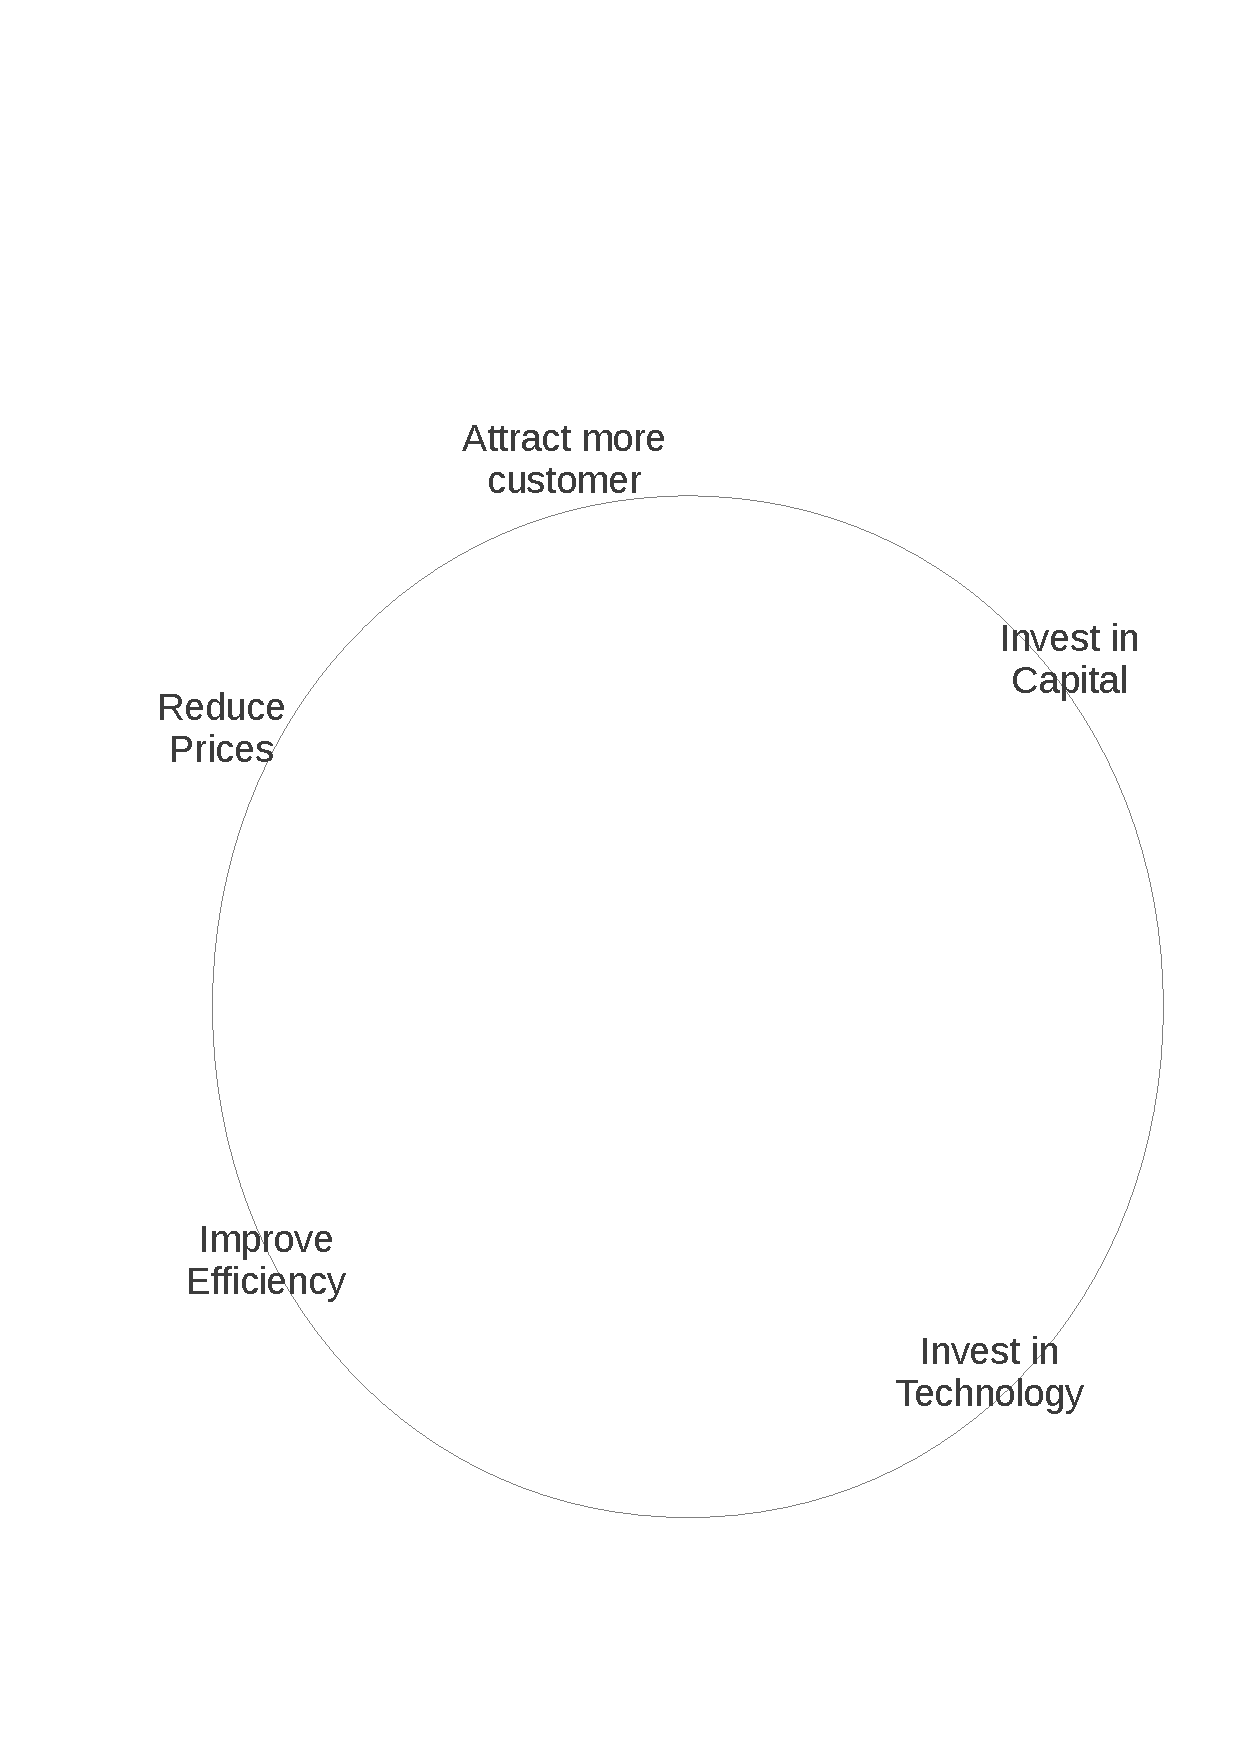
\includegraphics[width=0.5\textwidth]{./Figures/ScaleInnovation.pdf}
	\caption{Scale \& Innovation Drives Down Costs. Taken from~\cite{gavin2014ams}.}
	\label{fig:ScaleInnovation}
\end{figure}
\todo[inline]{Needs completing @ashleyjr}
